\documentclass{article} % For LaTeX2e
\usepackage{rickroll}
\usepackage{hyperref}
\usepackage{url}

\usepackage[left=1in, right=1in, top=1in, bottom=1in]{geometry}
\usepackage{mathexam}
 
%\ExamClass{COURSE NUMBER}
\ExamName{GitHub Token}
\ExamHead{}

\begin{document}

%\ExamNameLine

% Here is the header that adds all of the rickrolling commands
\rickroll

% You can add hidden questions as you would like
\hiddenquestion{How many licks does it take to get to the center of a Tootsie Pop?}

\ExamInstrBox{Before Beginning: I highly recommend creating a new GitHub Organization for each class, so that you don't have hundreds of repositories flooding your main account.  I also recommend getting verified for GitHub education \href{https://github.com/education/teachers}{Here}.
}

Using 

To create a Github authentification token, follw the steps below:

\begin{enumerate}
    \item Go to `github.com` and click on your image in the top right corner.\\
    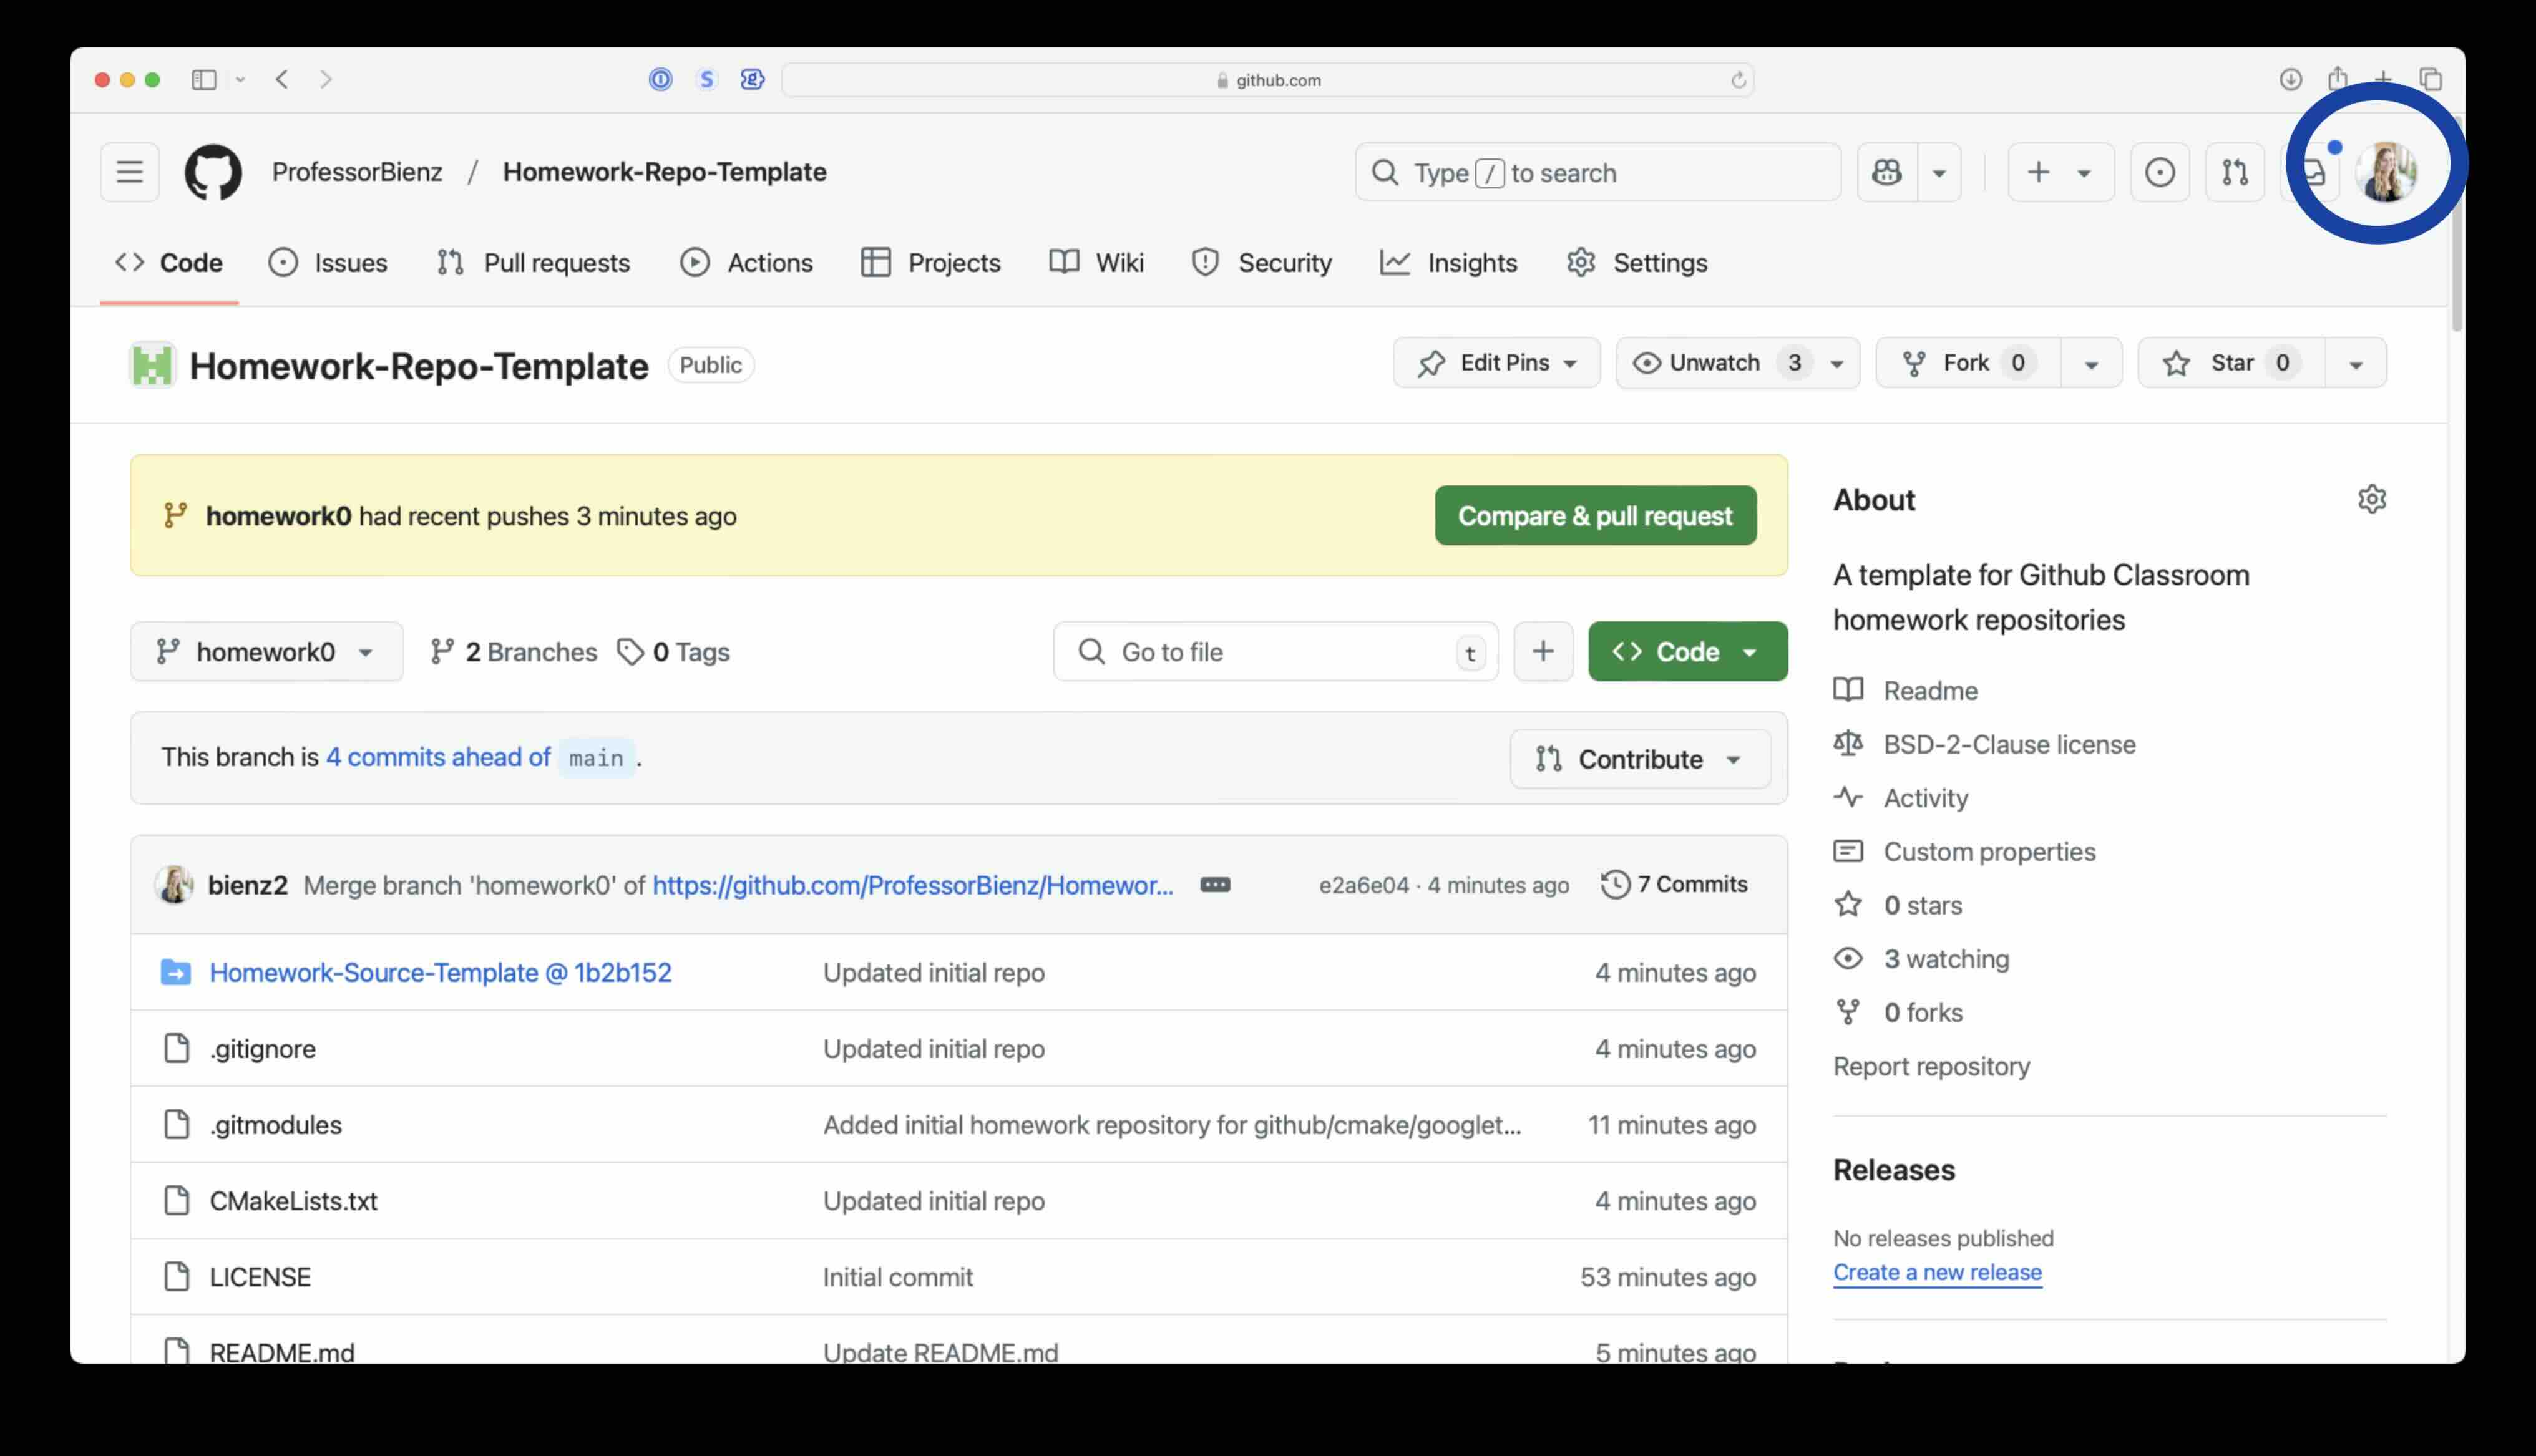
\includegraphics[width=0.75\textwidth]{figs/1picture.jpg}

    \item Click on `Settings`\\
    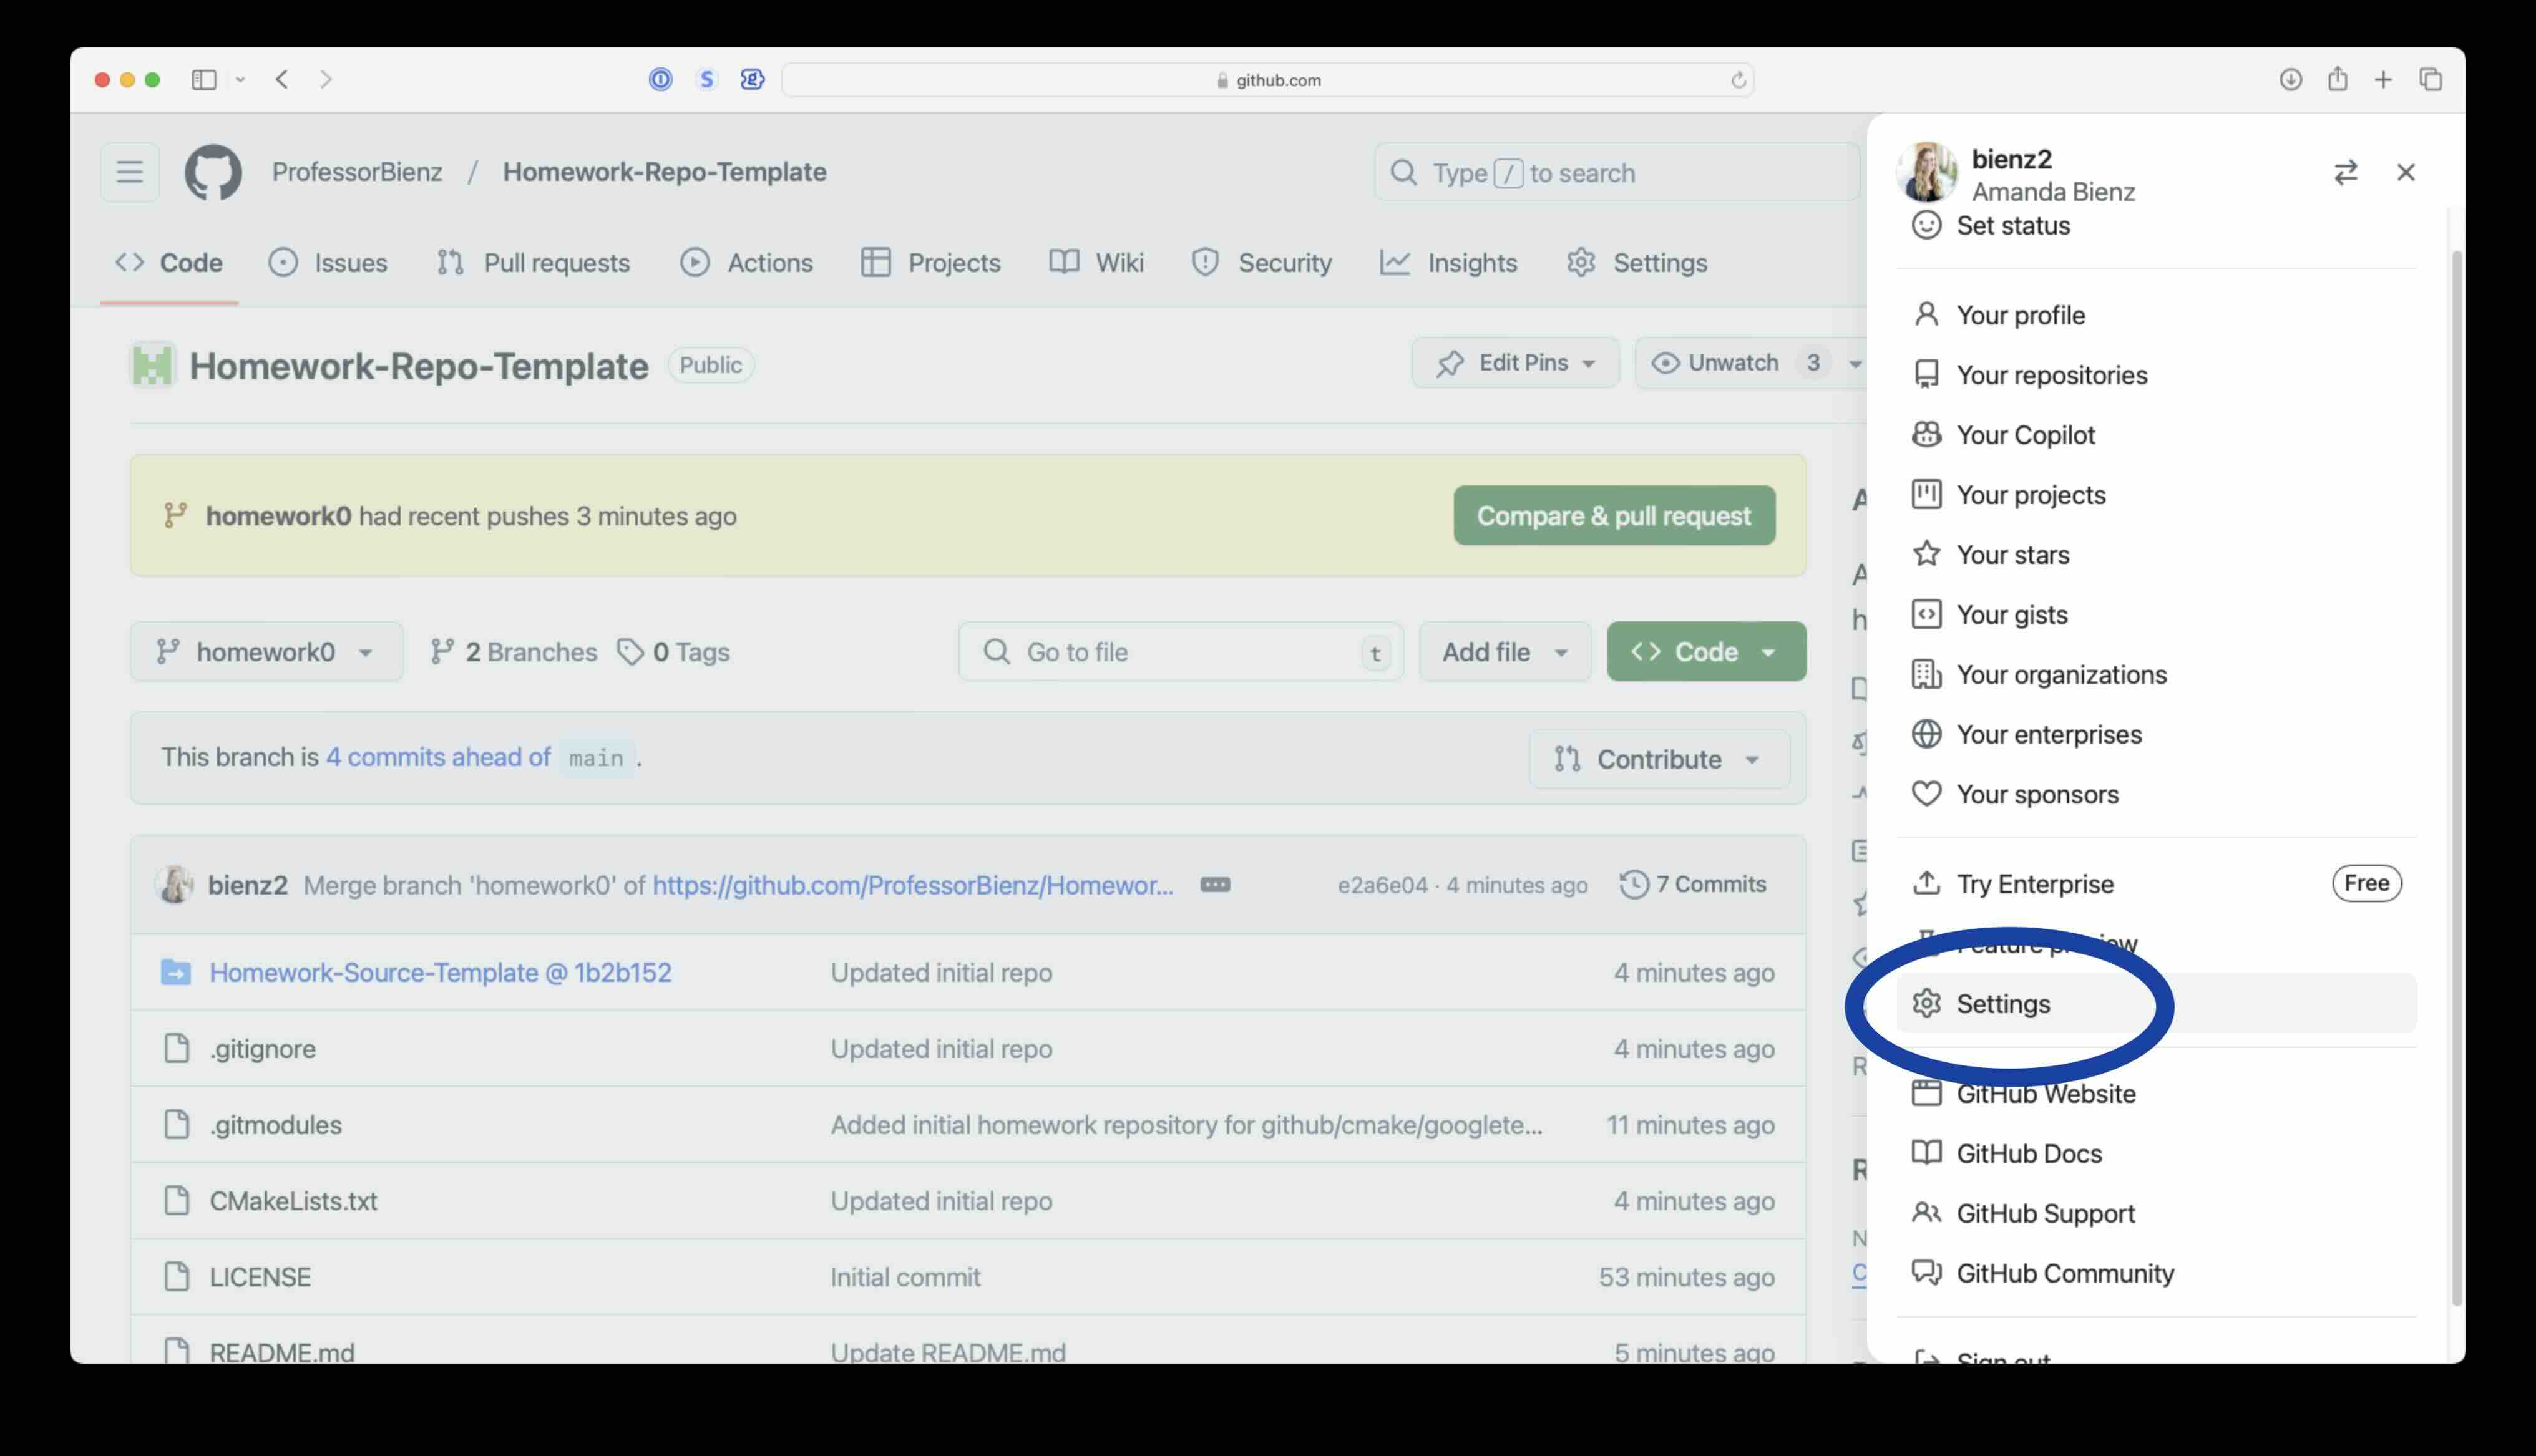
\includegraphics[width=0.75\textwidth]{figs/2settings.jpg}

    \item Scroll down and click on `Developer Settings`\\
    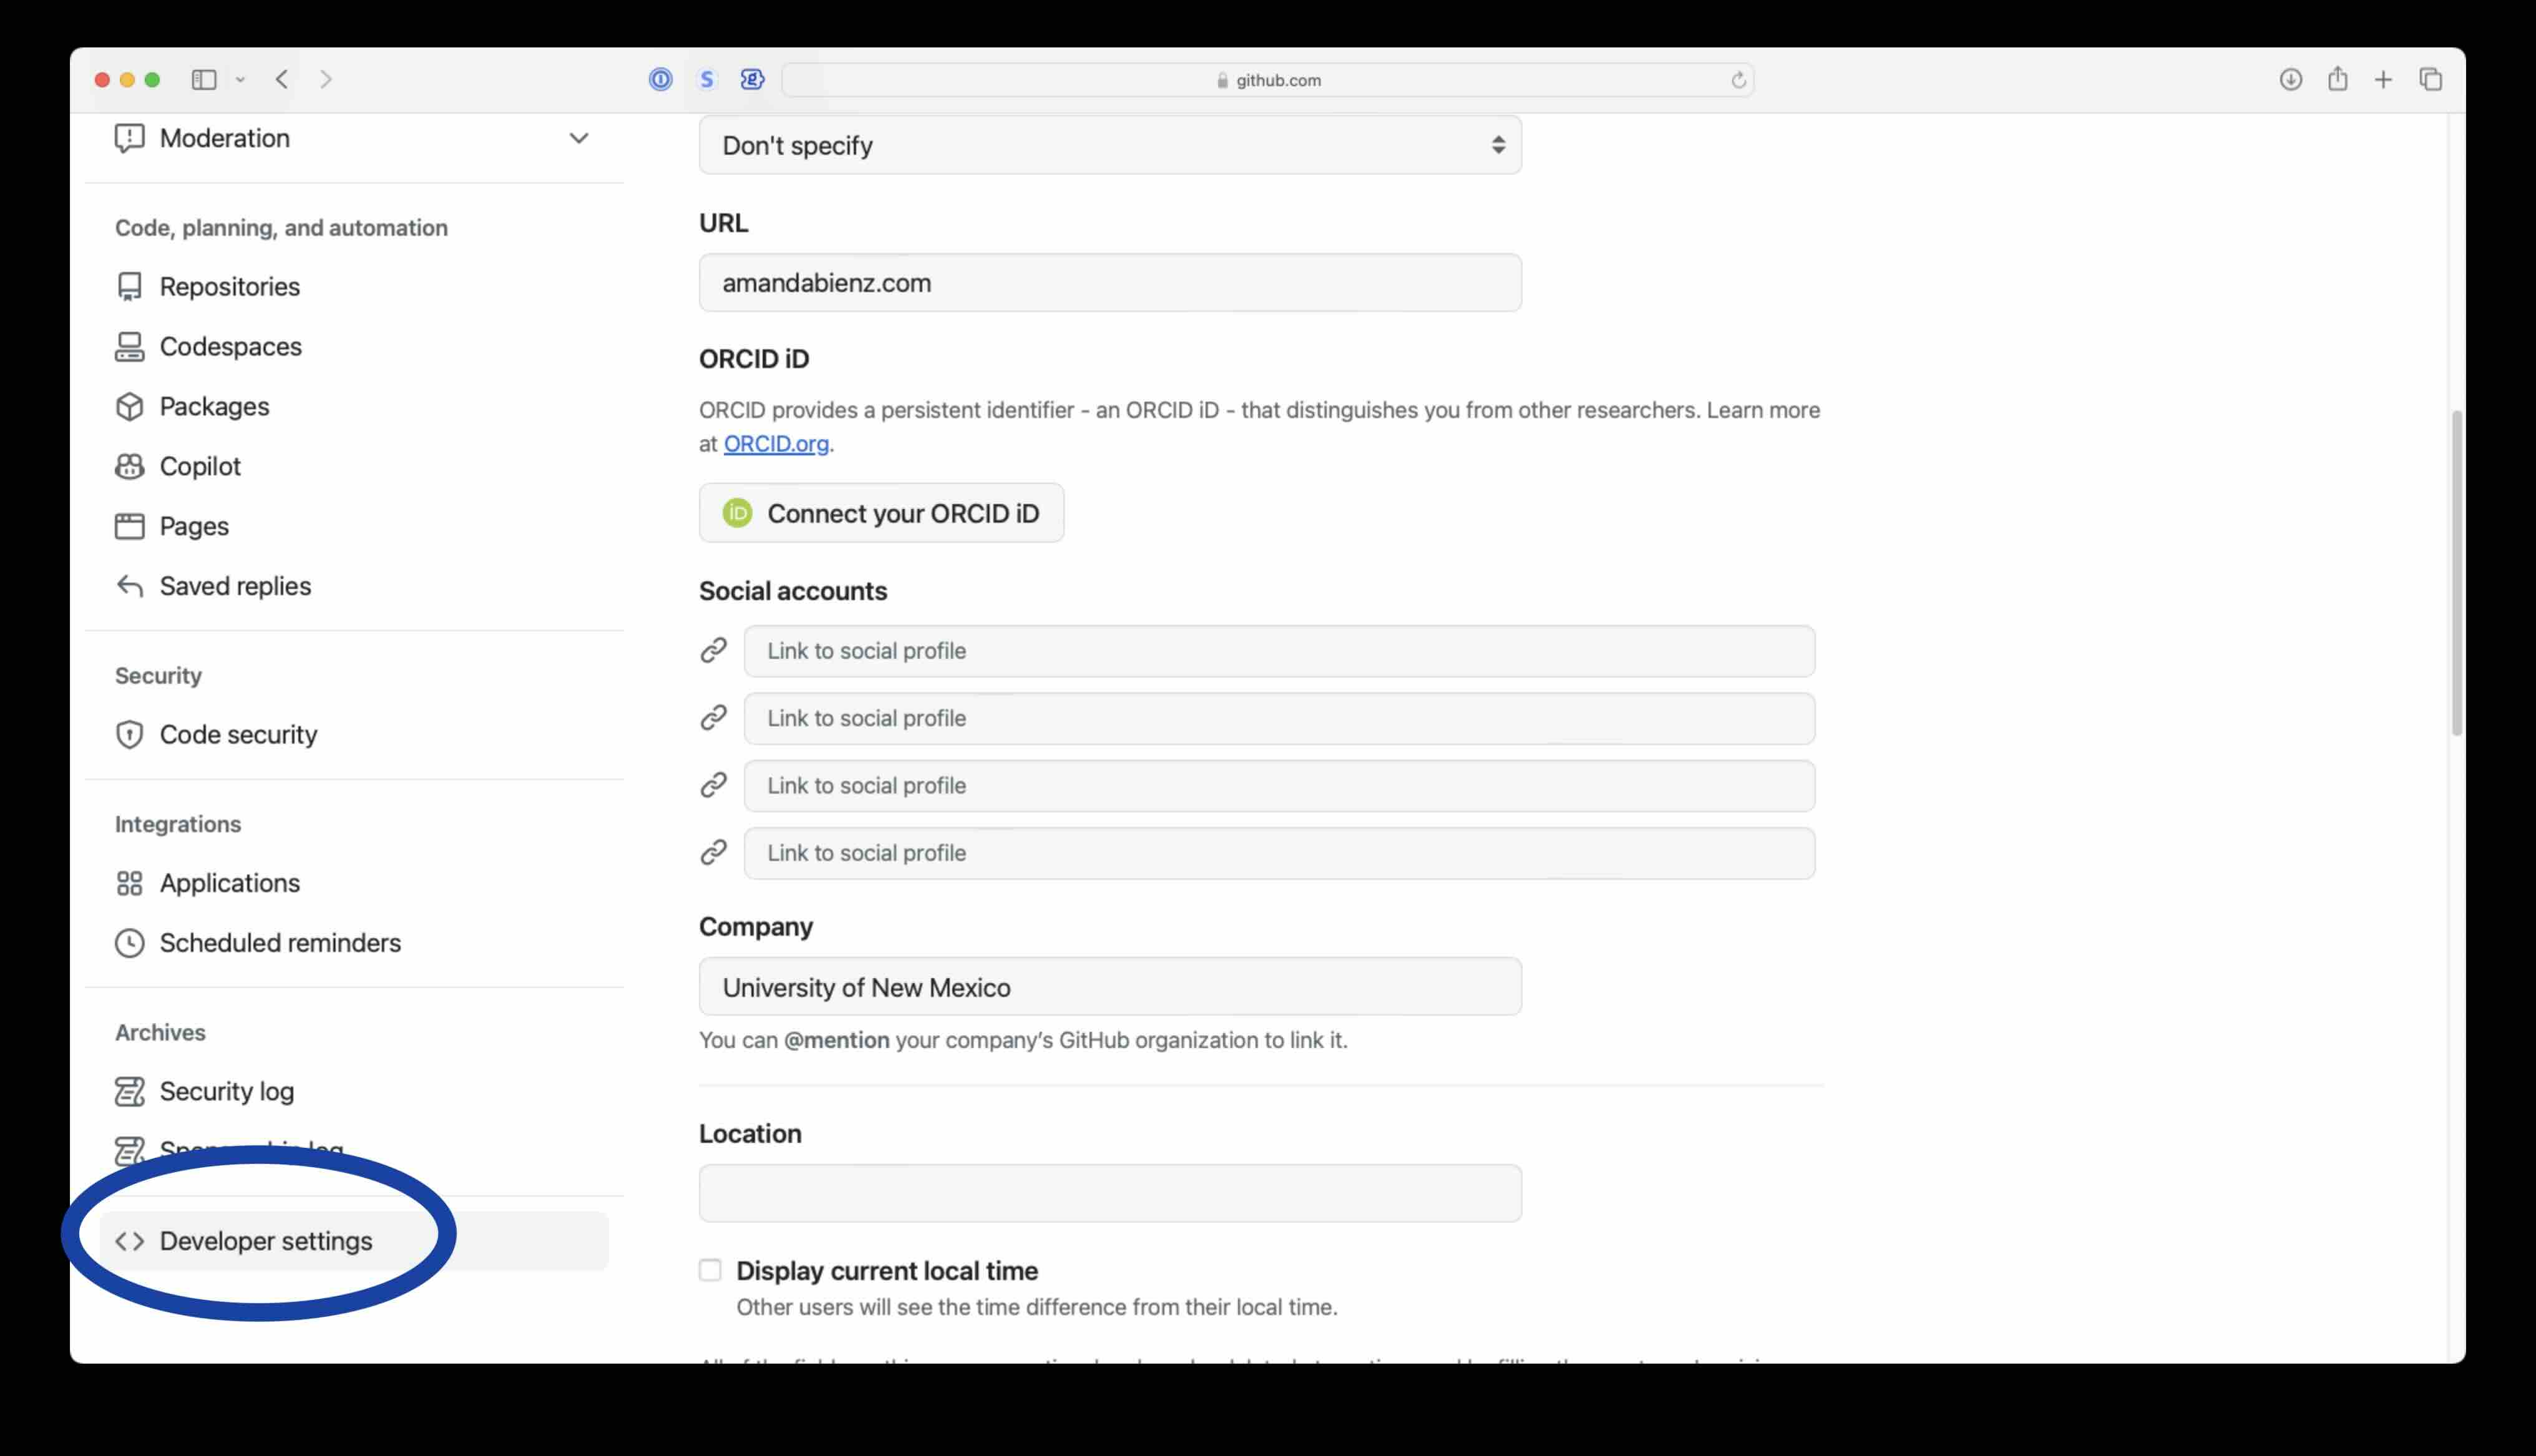
\includegraphics[width=0.75\textwidth]{figs/3developersettings.jpg}

    \item Click on `Personal Access Tokens` and `Tokens` (highlighted in blue).  Then click `generate new token` (both the green and then the red circles.\\
    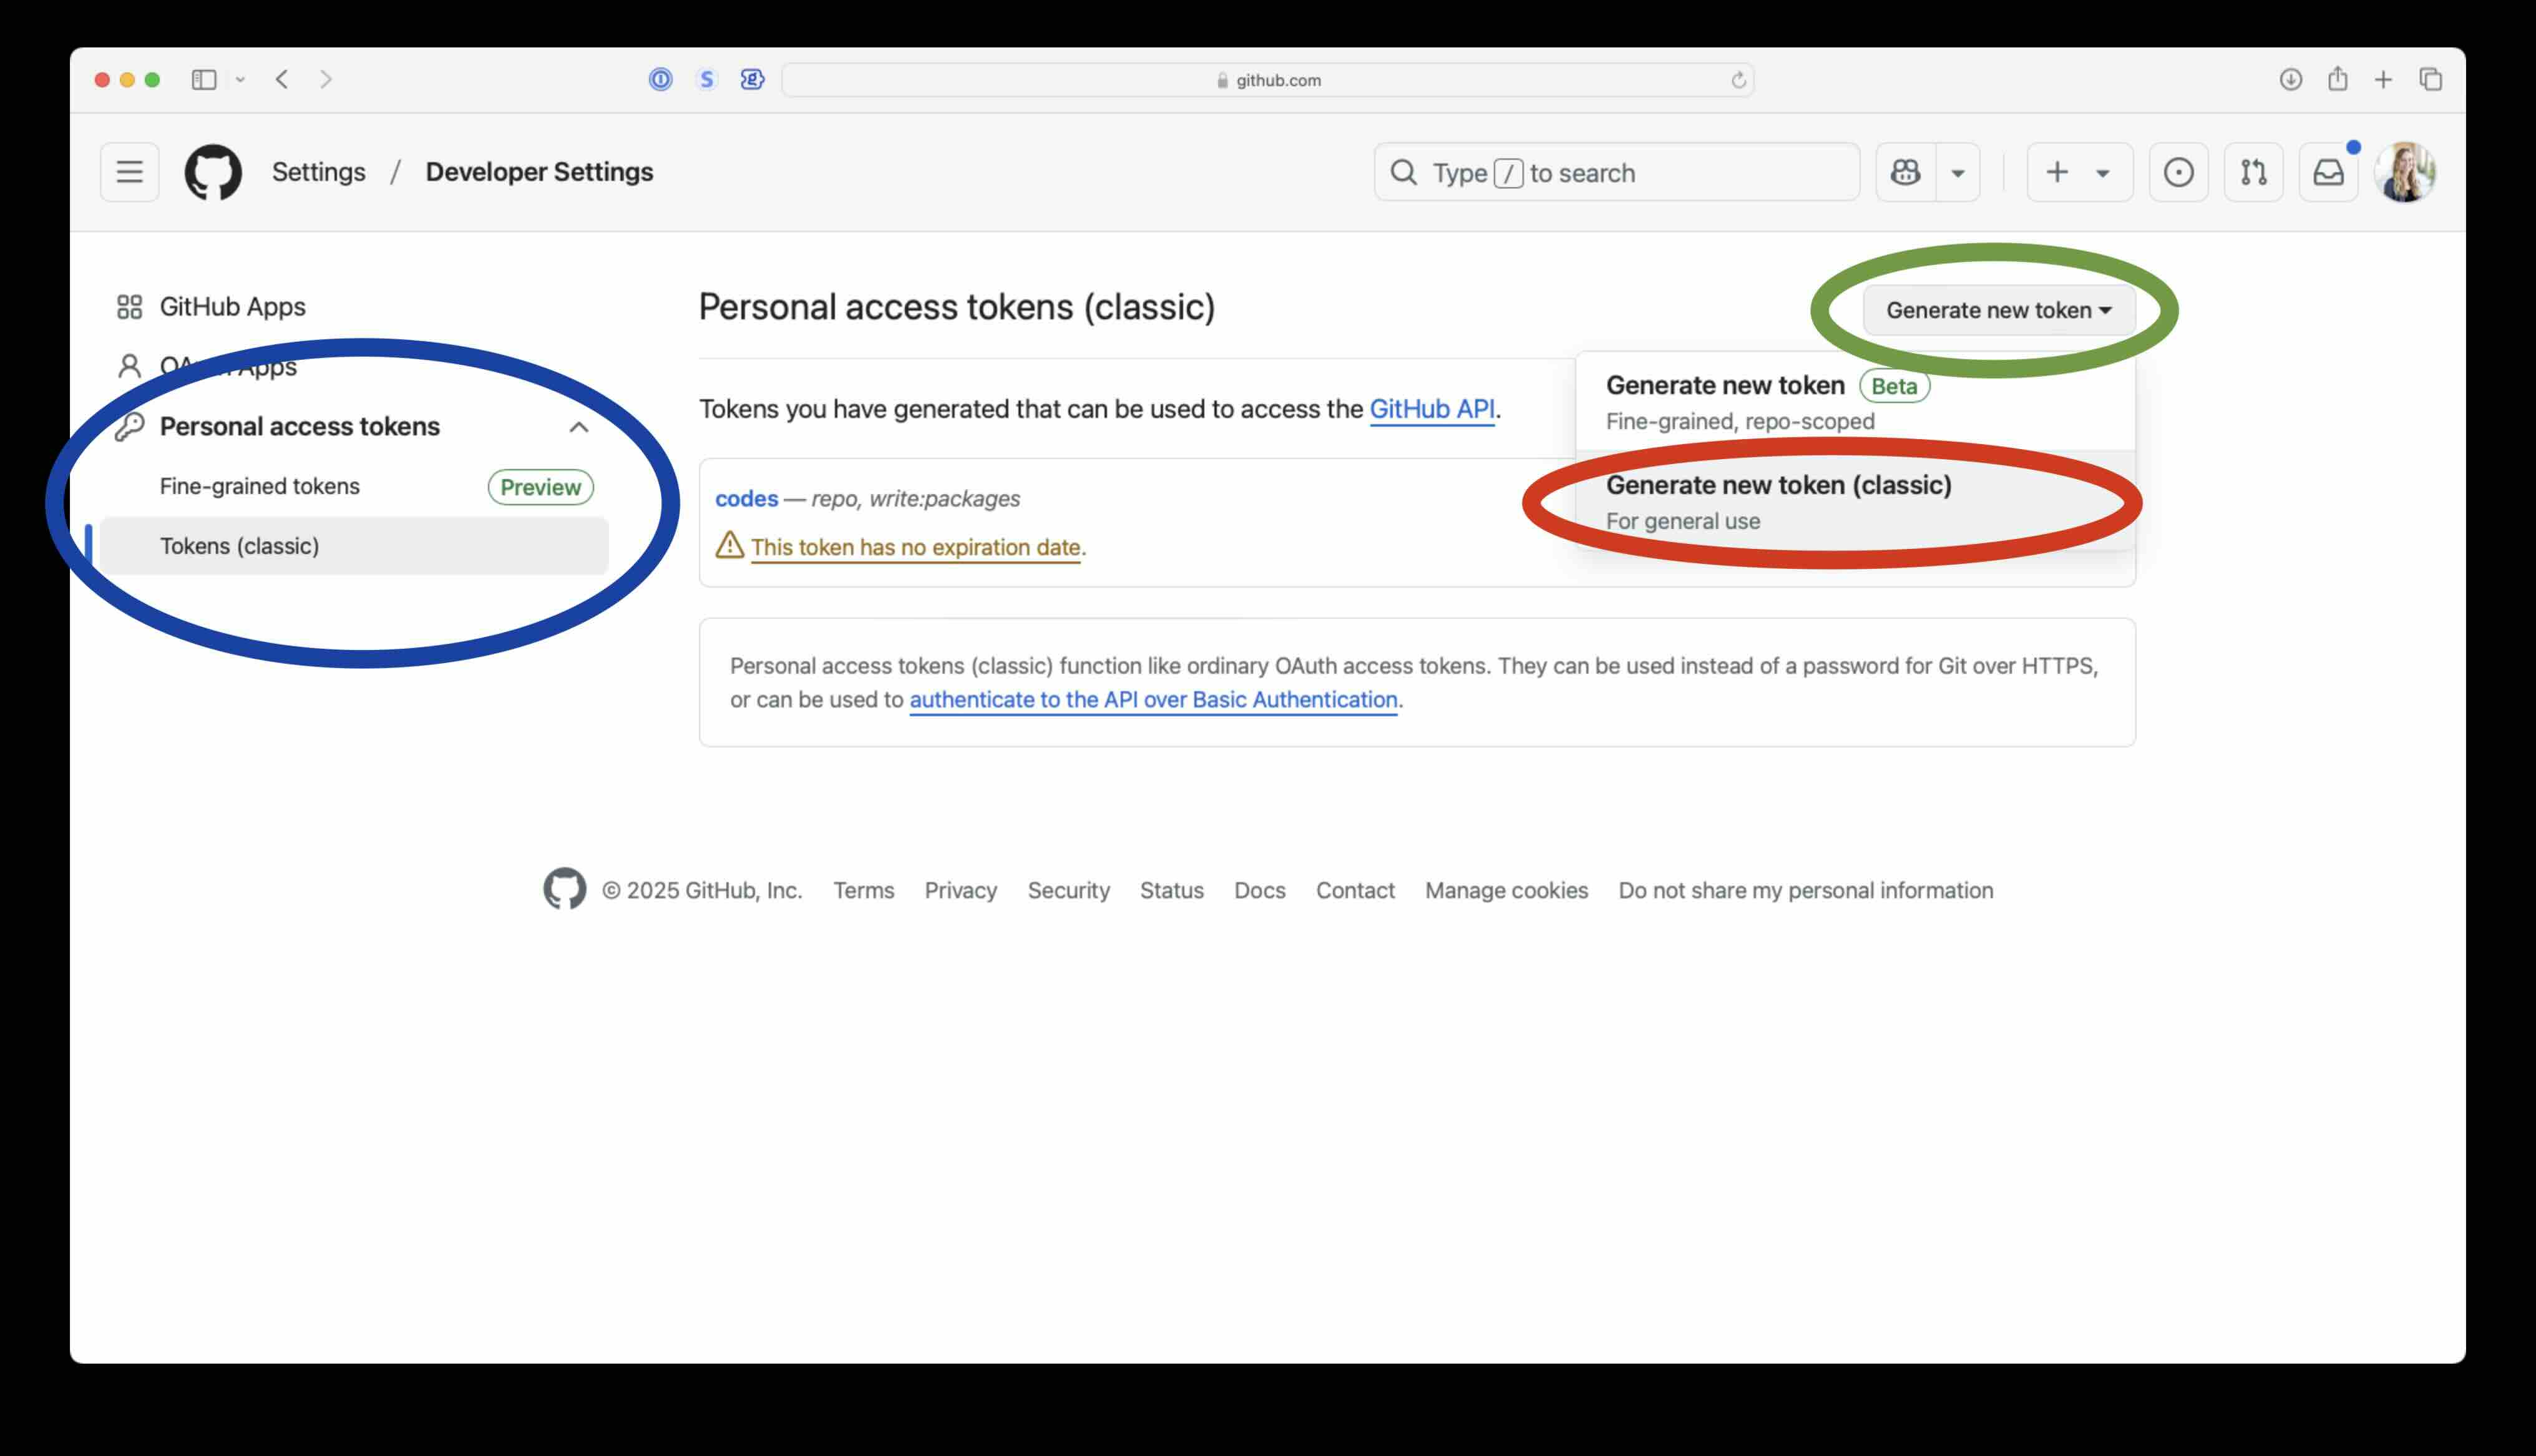
\includegraphics[width=0.75\textwidth]{figs/4createnew.jpg}

    \item This will allow you to create a new token.  Your token will be a generated password that will give you access to Github features.  To create a new token, give your token a name (green), select the amount of time your token should remain active (blue), and click the box next to `repo` (red).  The `repo` option lets you control code repositories.  \textbf{Make sure to select an expiration date past the end of the semester so that you don't need to redo these steps to complete assignments for the course.}\\
    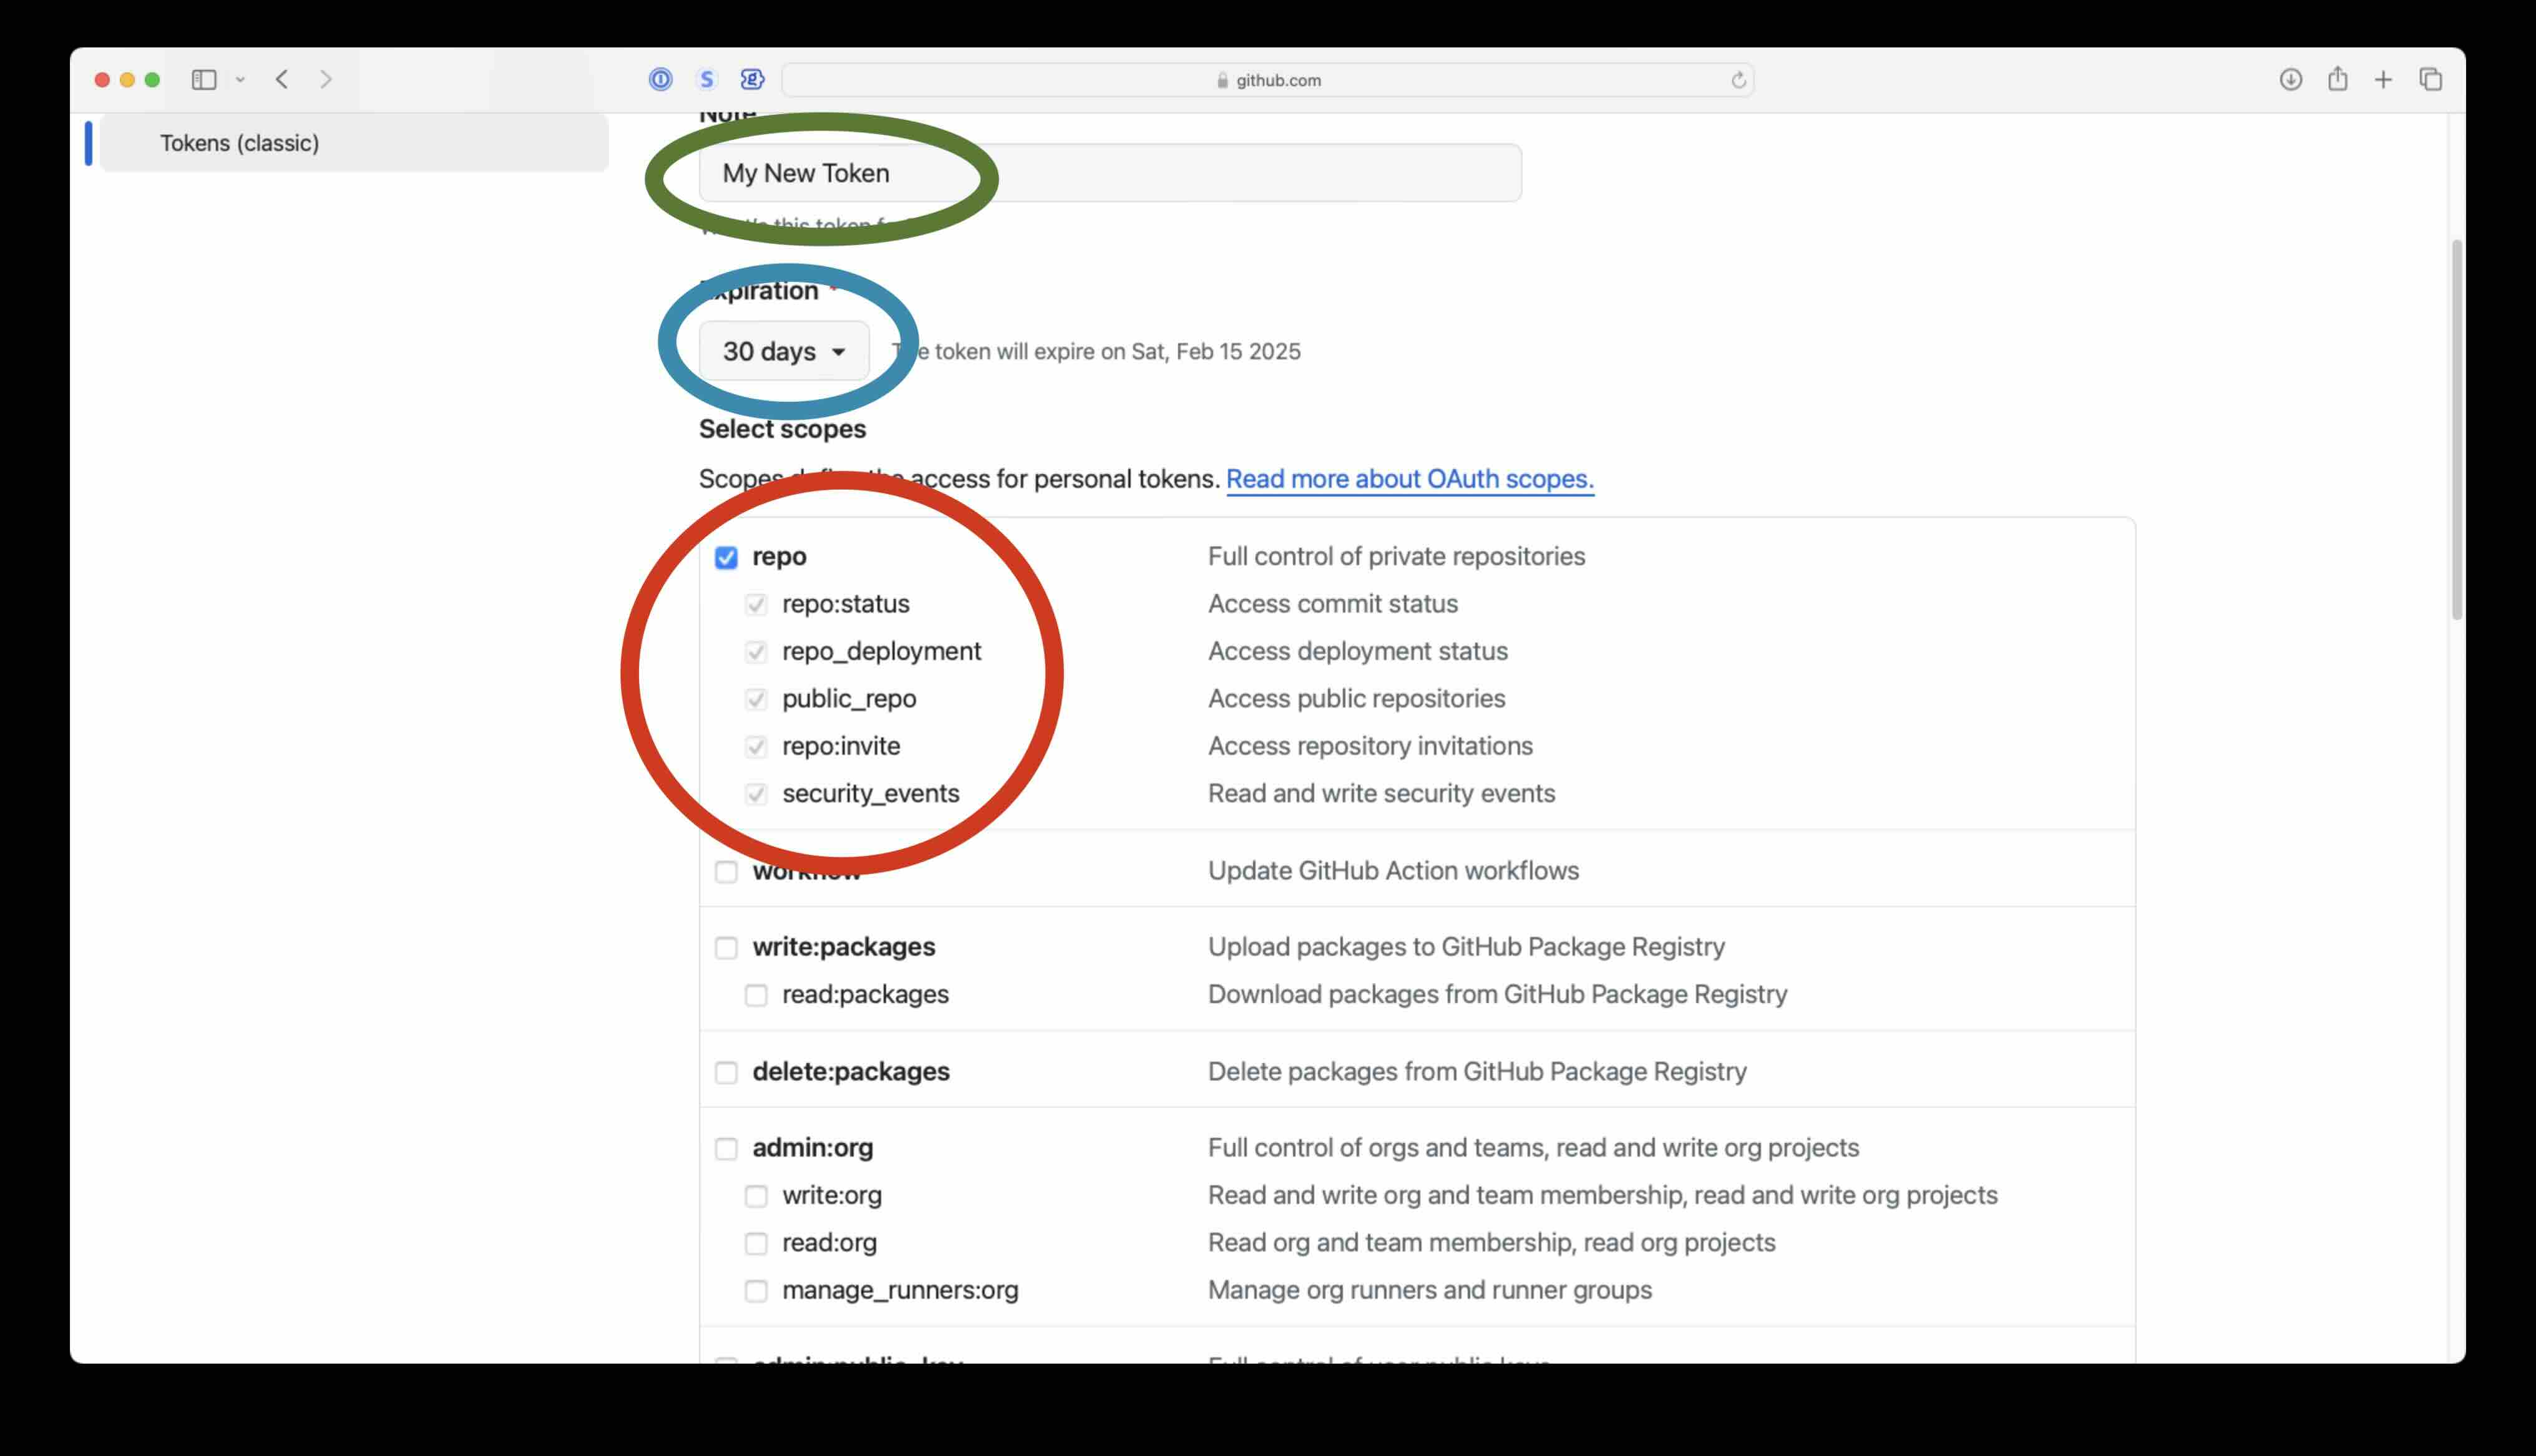
\includegraphics[width=0.75\textwidth]{figs/5token.jpg}

    \item Click `generate to create this token.\\
    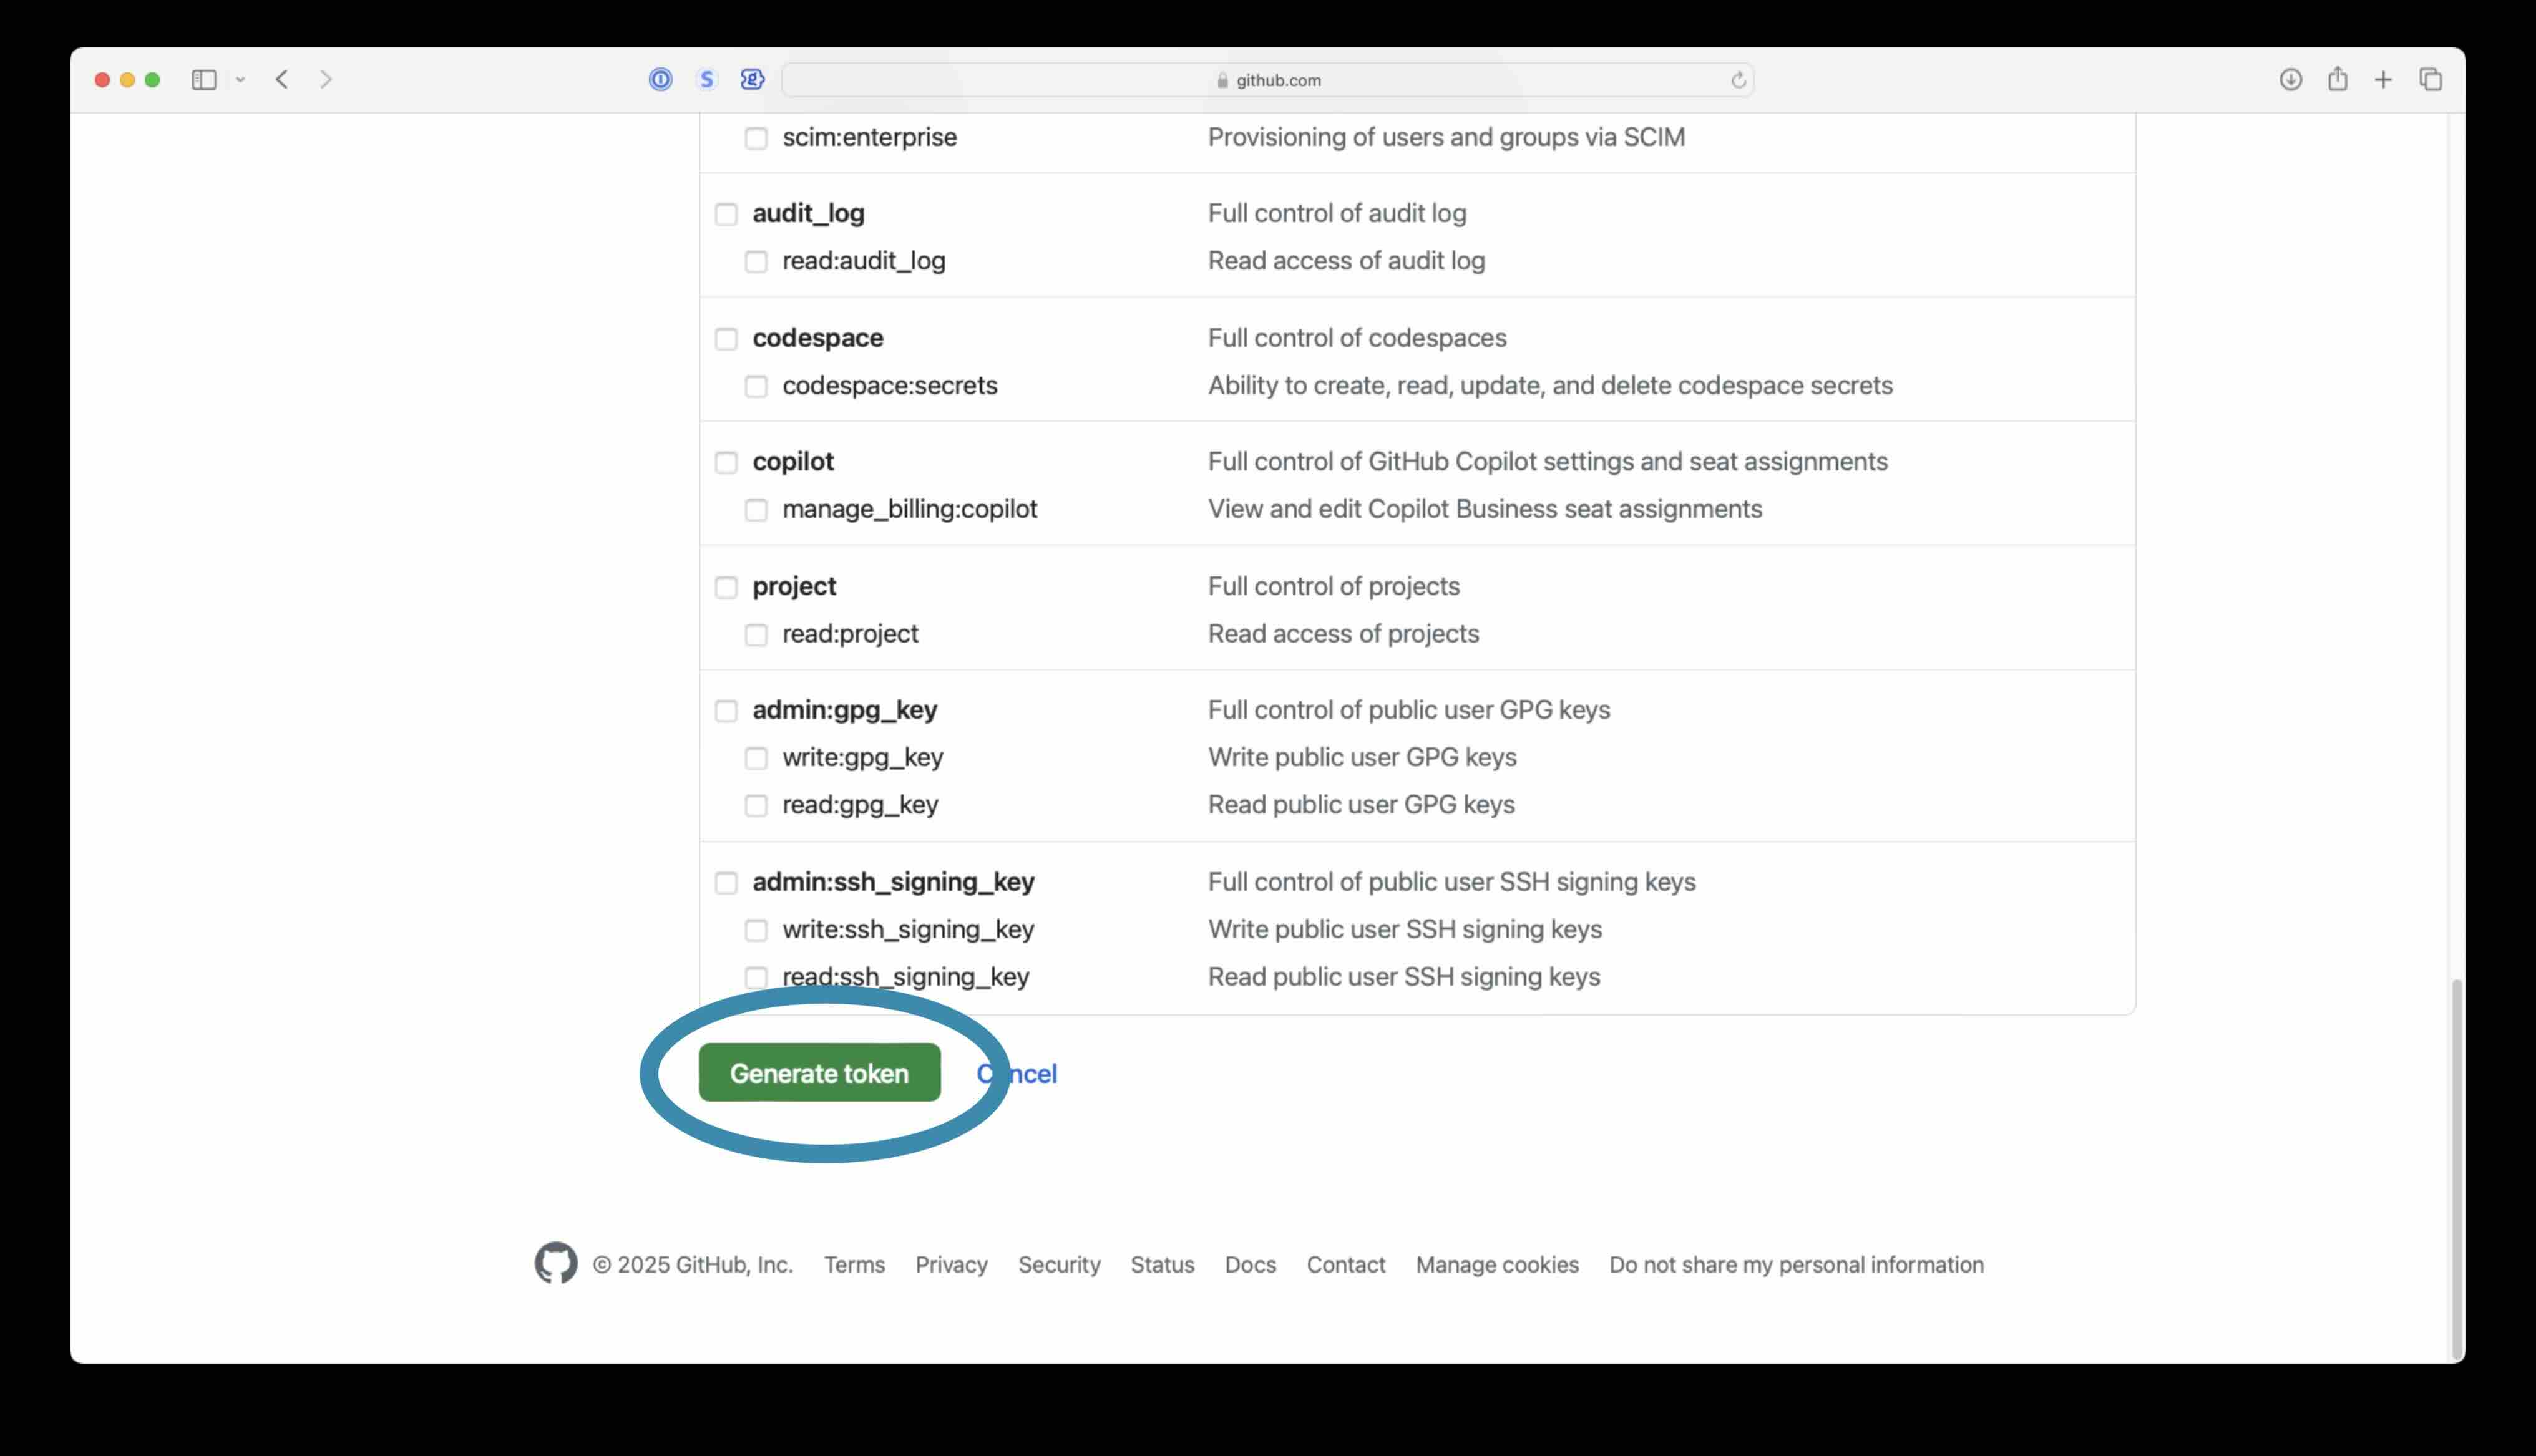
\includegraphics[width=0.75\textwidth]{figs/6generate.jpg}

    \item \textbf{You now have a token!}  It is a password, similar to that shown in the image below.  It will not allow you to login to `github.com`.  It will allow to `pull`, `push`, and otherwise manipulate homework repositories.\\
    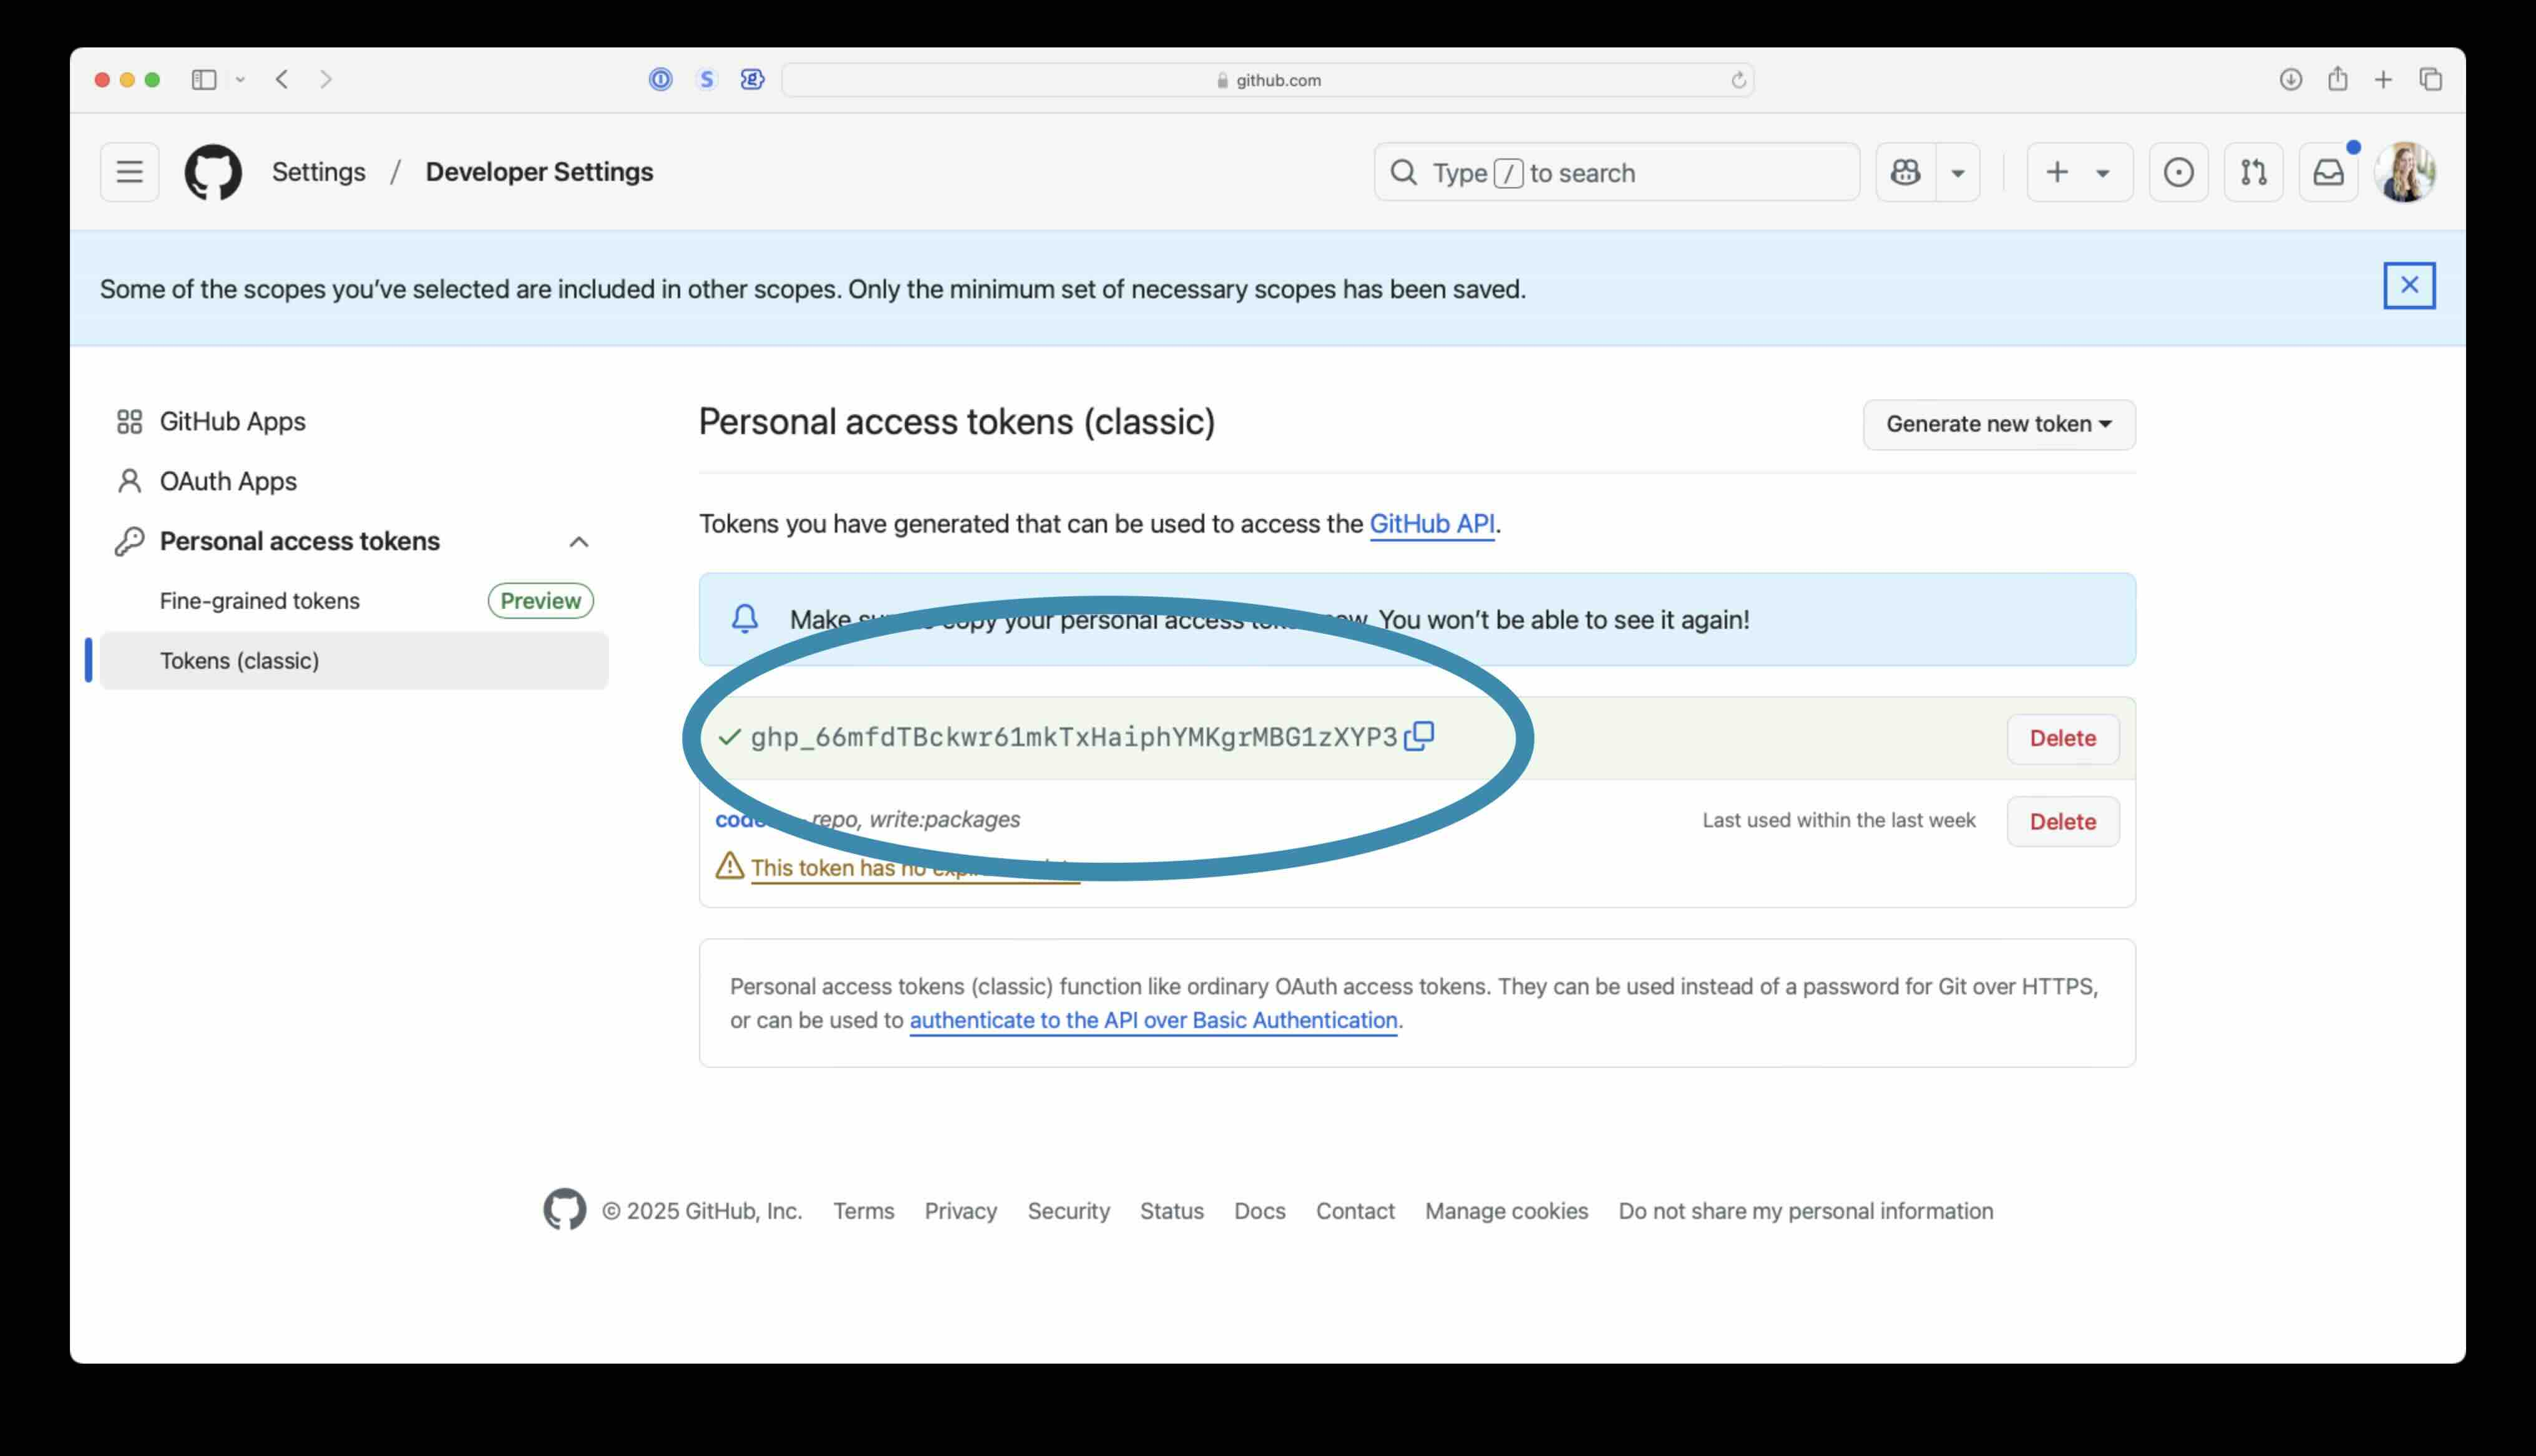
\includegraphics[width=0.75\textwidth]{figs/7password.jpg}
    
\end{enumerate}

\end{document}